% Modified for use with JCC - Madhusudan Singh Copyright (C) (2012). All rights reserved.
%\documentclass[12pt]{scrartcl}

\documentclass[12pt]{article}

\setlength{\oddsidemargin}{0in}  %left margin position, reference is one inch
\setlength{\textwidth}{6.5in}    %width of text=8.5-1in-1in for margin
\setlength{\topmargin}{-0.5in}    %reference is at 1.5in, -.5in gives a start of about 1in from top
\setlength{\textheight}{9.1in}     %length of text=11in-1in-1in (top and bot. marg.) 
\newenvironment{wileykeywords}{\textsf{Keywords:}\hspace{\stretch{1}}}{\hspace{\stretch{1}}\rule{1ex}{1ex}}

\usepackage{amsmath,amssymb,txfonts,bm}
\usepackage{feynmf}
\usepackage{graphicx,xstring}% Include figure files

%\usepackage{caption}
\usepackage{color}% Include colors for document elements
\usepackage{dcolumn}% Align table columns on decimal point
\usepackage{bm}% bold math
\usepackage[numbers,super,comma,sort&compress]{natbib}
%\usepackage[nolists, nomarkers, figuresfirst]{endfloat}
\usepackage{booktabs}

\usepackage{relsize}
\let\acr=\textsmaller

\frenchspacing

\definecolor{background-color}{gray}{0.98}

\newcommand{\onlinecite}[1]{\!\citenum{#1}}

% Include or exclude figures in the latexing 
%\newcommand{\slow}[1]{}
\newcommand{\slow}[1]{#1} 

% For some reason, vertical alignment in tables with includegraphics doesn't work without this
\newcommand{\tableimage}[2]{\begin{tabular}{c} \includegraphics[width=#1]{#2} \end{tabular}} 
\newcommand{\transitionrightarrow}{\tableimage{1cm}{fat-rightarrow}}
\newcommand{\transitiondownarrow}{\tableimage{1cm,angle=-90}{fat-rightarrow}}
\newcommand{\transitionuparrow}{\tableimage{1cm,angle=90}{fat-rightarrow}}

\renewcommand{\thefootnote}{\fnsymbol{footnote}}

%\bibliographystyle{apsrev_no_url}
%\bibliographystyle{ijqc}
\bibliographystyle{diy-WIRE}

\title{The Dirac Equation in Electronic Structure Theory}

%Author sequence to be decided after finishing the paper (PS I personally don't care which way)
\author{Peter Schwerdtfeger,$^*$ Luk\'a\v{s} F. Pa\v{s}teka\thanks{Centre of Theoretical Chemistry and Physics, The New Zealand Institute for Advanced Study, 
Massey University Auckland, Private Bag 102904, 0632 Auckland, New Zealand. Email: \texttt{p.a.schwerdtfeger@massey.ac.nz}},
~and Trond Saue\thanks{Laboratoire de Chimie et Physique Quantiques UMR 5626 CNRS --- Universit\'e Toulouse III-Paul Sabatier 118 route de Narbonne, 31062 Toulouse (FRANCE). Email: \texttt{trond.saue@irsamc.ups-tlse.fr}}
}

\begin{document}

\maketitle

%abstract
\begin{abstract}
The Dirac equation applied in relativistic electronic structure theory is introduced and discussed in detail
including transformations to two-component forms and corresponding picture change effects for properties.
Recent progress in bound-state quantum electrodynamics and its importance to accurate electronic structure
theory is analyzed. A short discussion on the current standard model and the search for new physics is also presented.
Few applications are presented using prime examples for the importance of relativistic and quantum electrodynamic
effects in heavy element chemistry. Special emphasis is put on the many theoretical and technical difficulties 
in treating the Dirac equation and quantum electrodynamic effects.
\end{abstract}

\begin{wileykeywords}
Dirac equation; two-component forms; bound state quantum electrodynamics; standard model and beyond; relativistic and QED effects.
\end{wileykeywords}

%*****************Graphical Table of Contents******************** THIS IS MANDATORY *******************

\slow{
\begin{figure}[h]
\centering
%\colorbox{background-color}
{
\fbox{
\begin{minipage}{0.60\textwidth}
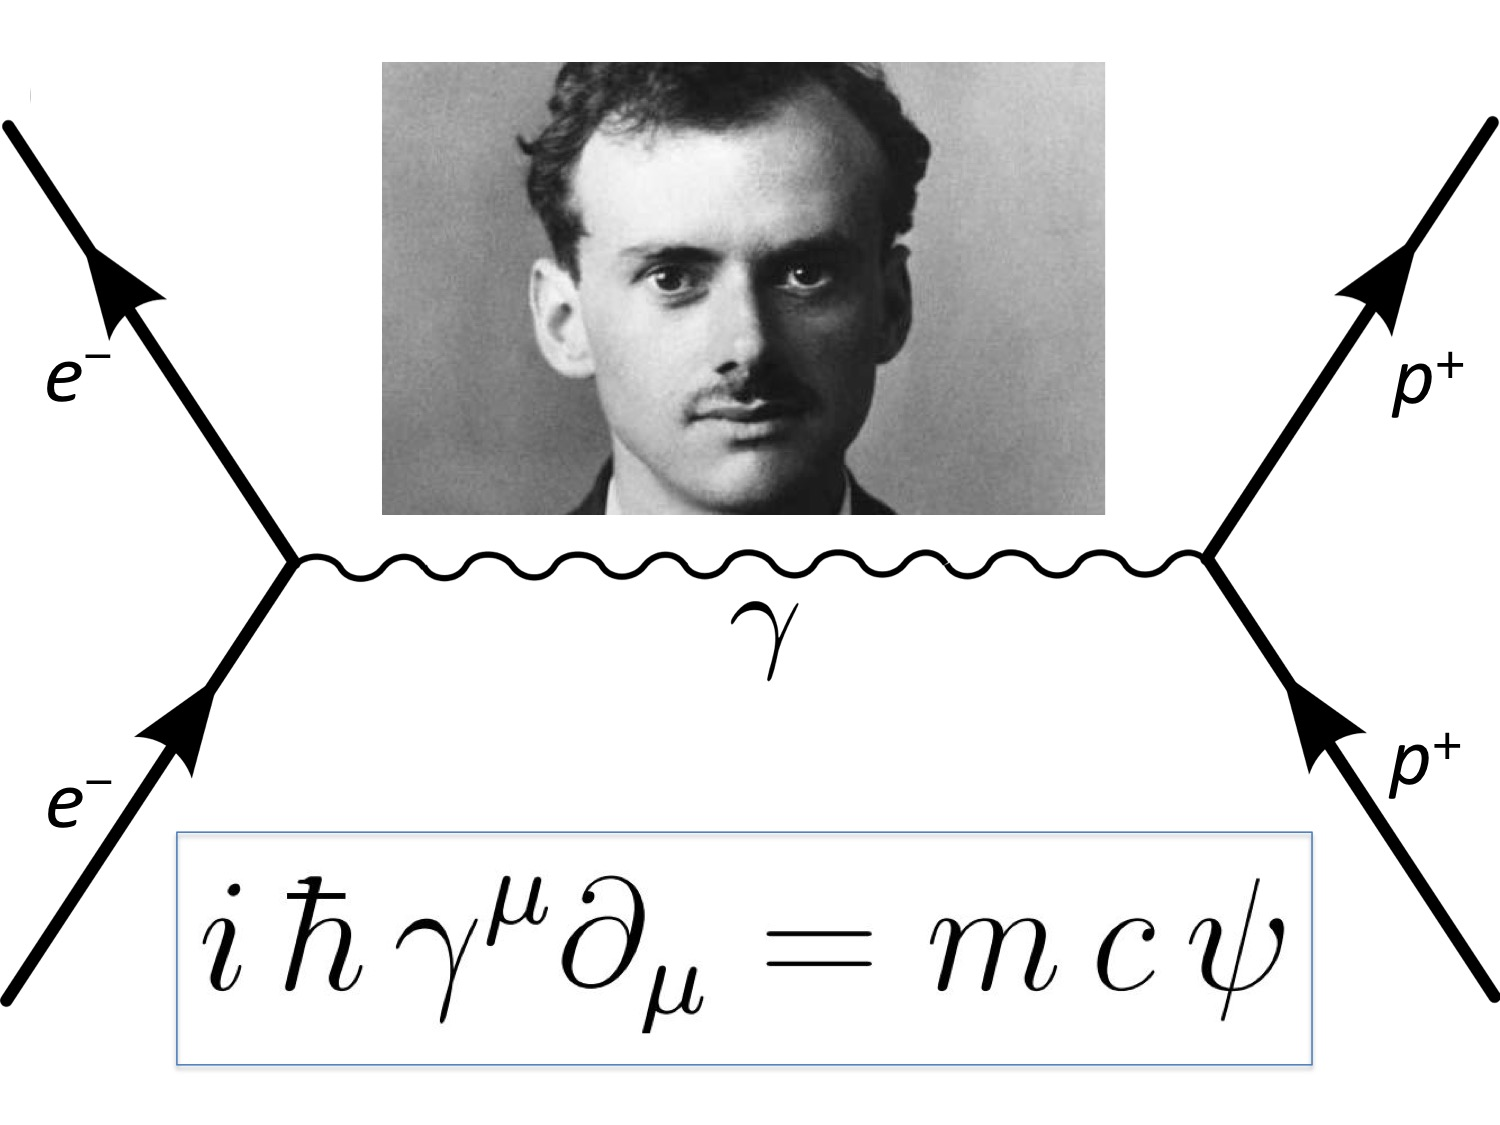
\includegraphics[height=75mm]{TOC.jpg}\\
\centering
Table of Content Picture
\end{minipage}
}
}
\end{figure}
}

% makes references listed with 1., 2., etc.  
  \makeatletter
  \renewcommand\@biblabel[1]{#1.}
  \makeatother


\renewcommand{\baselinestretch}{1.5}
\normalsize


\clearpage
\linespread{1.2}

%INTRODUCTION
\section{\sffamily \Large INTRODUCTION}

In 1928, P. A. M. Dirac proposed a relativistic formulation for the quantum theory of a spin 1/2 particle with rest mass $m$ in external scalar $V(\vec{r},t)$ and vector $\vec{A}(\vec{r},t)$ fields,\cite{Dirac-1928,Dirac-1929,Dirac-1930}
\begin{equation}
   i \hbar \frac{\partial}{\partial t} \Psi (\vec{r},t) = \left\{ c \vec{\alpha} \left(\vec{p} + \frac{e}{c}\vec{A}(\vec{r},t) \right) + \beta mc^2 + V(\vec{r},t) \right\} \Psi (\vec{r},t)
   \label{Dirac1}
\end{equation}
with the velocity of light set at $c$ = 299792458 ms$^{-1}$. In Dirac's formulation fermionic spin emerges naturally as a consequence of a relativistic treatment by enforcing Lorentz invariance, and
in a complete covariant formulation it reads,\footnote{We keep this review short and without any proofs to not distract from the main important facts, and more complicated mathematical issues are moved into the footnotes. When appropriate, references are given for a more detailed treatment.}$^,$\footnote{Common (3-)vectors $\vec{v}\in V(\mathbb{R}^3)$ are used here with a vector sign, and 4-vectors (Lorentz vectors) $x_\mu=(ict,x_1,x_2,x_3) \in \mathcal{M} ~(\mu = 0,1,2,3)$ in Minkowski space $\mathcal{M}$ are used with Greek subscript symbols. The Einstein sum convention for repeated indices in products of 4-vectors/tensors are used. We note that in special relativity we do not need the more commonly used formulation of co- and contra-variant vectors in physics (which requires the introduction of a dual space), which is more important in the theory of general relativity.}
\begin{equation}
   \left\{ mc + \hbar\gamma_\mu \partial_\mu \right\} = 0
   \label{Dirac2}
\end{equation}
with the external potential being introduced by minimal coupling (also called minimal substitution),
\begin{equation}
   p_\mu \mapsto p_\mu - \frac{q}{c}A_\mu
   \label{MinCoup}
\end{equation}
with the charge $q=-e$ for an electron ($e$ is the elementary charge), and $\partial_\mu=\frac{\partial}{\partial x_\mu}$. Here $\vec{\alpha}$, $\beta$ and $\gamma_\mu=(\beta,-i\beta\gamma_1,-i\beta\gamma_2,-i\beta\gamma_3)$ are the Dirac $(4\times 4)$ matrices in standard representation,
\begin{equation}
   \vec{\alpha} = \left( \begin{matrix} 0 & \vec{\sigma}  \\ \vec{\sigma} & 0  \end{matrix} \right) \quad,\quad
   \beta = \gamma_0 = \left( \begin{matrix} 1 & 0  \\ 0 & -1  \end{matrix} \right) \quad,\quad
   \vec{\gamma} = -i\beta\vec{\alpha} = i \left( \begin{matrix} 0 & -\vec{\sigma}  \\ \vec{\sigma} & 0  \end{matrix} \right)
   \label{DiracMatrix}
\end{equation}
and $\vec{\sigma}$ are the $(2\times 2)$ Pauli spin matrices,
\begin{equation}
   \sigma_1 = \left( \begin{matrix} 0 & 1  \\ 1 & 0  \end{matrix} \right) \quad,\quad
   \sigma_2 = \left( \begin{matrix} 0 & -i  \\ i & 0  \end{matrix} \right) \quad,\quad
   \sigma_3 = \left( \begin{matrix} 1 & 0  \\ 0 & -1  \end{matrix} \right) \quad,\quad
   \label{PaulMatrix}
\end{equation}

Why should we use the Dirac equation in electronic structure theory instead of the Schr\"odinger equation, as the latter has served the quantum chemical community extremely well for almost a century. We may rightly ask {\it what is wrong with the Schr\"odinger equation}, or, {\it why do we have to turn to the more complicated Dirac equation} known to be not without difficulties?\footnote{Unlike the semi-bound nonrelativistic Schr\"odinger operator $\hat{H}$, the relativistic Dirac operator $\hat{D}$ is unbound requiring extra boundary conditions in a variational treatment. Moreover, it requires the introduction of a finite nuclear charge to keep $\hat{D}$ self-adjoint beyond nuclear charge 137.} From a purely theoretical view point the answer is simple: In the Schr\"odinger picture the time-evolution is given by the unitary transformation
\begin{equation}
   \Psi (t) = U(t-t_0) ~\Psi (t_0) = e^{-i\hat{H}(t-t_0)/\hbar} ~\Psi (t_0)
   \label{timeevo}
\end{equation}
(related to Stone's theorem\footnote{Stone's theorem is a basic theorem of functional analysis that establishes a one-to-one correspondence between self-adjoint operators on a Hilbert space $\mathcal{H}$ to one-parameter families of unitary operators that are strongly continuous. This defines the derivative of the mapping $t\mapsto Ut$, which is only supposed to be continuous.}) leading to the Schr\"odinger equation
\begin{equation}
   i \hbar \frac{\partial}{\partial t} \Psi (t) = \hat{H} \Psi (t)
   \label{Schrodinger}
\end{equation}
If we accept the first derivative in time as being fundamental, we strictly require first derivatives in space to enforce (relativistic) Lorentz invariance. The Schr\"odinger equation is, however, {\it not} Lorentz invariant as space derivatives appear in second instead of first order,
\begin{equation}
   i \hbar \frac{\partial}{\partial t} \Psi (\vec{r},t) = \left[ -\frac{\hbar^2}{2\mu} \Delta + V(\vec{r},t)\right] \Psi (\vec{r},t)
   \label{Schrodinger1}
\end{equation}
This may not be seen as an important drawback if nonrelativistic particles are involved,\footnote{We define a particle to behave nonrelativistically if its interaction energy $E_{int}$ with an external field (such as the Coulomb field of a nucleus) is much less than the particle's rest mass energy, i.e. $E_{int}<<mc^2$. For an electron the rest mass energy is $m_ec^2$=510.998910(13) keV which can be compared for example to the K-shell ionization potential of Pb with 88 keV.} but the Schr\"odinger equation is also ``spin-free'', e.g. the Schr\"odinger operator $\hat{H}$ does not contain terms accounting for fine-structure effects for a spin 1/2 particle which becomes large in heavy elements, and experimentally observed fine (and hyperfine) splittings in atoms and molecules cannot be reproduced. If the spin of a particle is introduced into a (nonrelativistic) Galilei-invariant formalism, the resulting L\'evy-Leblond equation leads to an incorrect spin-orbit coupling term.\cite{levy-leblond-1967} If spin interaction terms like the spin-orbit operator are introduced ad-hoc into the Schr{\"o}dinger equation, the specific form of this operator still requires theoretical justification, and this can only be done through the Dirac equation (see section \ref{TwoComp} on two-component forms). 
We also know that for heavy elements the Schr{\"o}dinger equation yields results for inner shell ionization potentials that seriously deviate from experimental values. This may, however, not impress chemists and we may still ask why relativistic effects should be of any importance to valence electrons, as the interaction energy of an electron with a positively charged (but screened) nucleus is only in the eV range and much less compared to the electron's rest mass energy.

Dirac stated in 1929\cite{Dirac-1929} that relativistic effects are not important to chemistry as valence electrons move rather slowly compared to the velocity of light, and similar statements were made not too long ago.\footnote{Dirac's statement in 1929 reads\cite{Dirac-1929} {\it The general theory of quantum mechanics is now almost complete, the imperfections that still remain being in connection with the exact fitting of the theory with relativity ideas. These gives rise to difficulties only when high-speed particles are involved, and are therefore of no importance in the consideration of atomic and molecular structure and ordinary chemical reactions, in which it is, indeed, usually sufficiently accurate if one neglects relativity variation of mass with velocity and assumes only Coulomb forces between the various electrons and atomic nuclei.} Even in 1988 Glashow wrote\cite{glashow-1993} {\it Modern elementary-particle physics is founded upon the two pillars of quantum mechanics and relativity. I have made little mention of relativity so far because, while the atom is very much a quantum system, it is not very relativistic at all. Relativity becomes important only when velocities become comparable to the speed of light. Electrons in atoms move rather slowly, at a mere one percent of light speed. Thus it is that a satisfactory description of the atom can be obtained without Einstein's revolutionary theory.} However, as early as in 1932 Vallarta and Rosen stated that\cite{Vallarta-1932} {\it While this [relativistic] correction may be expected to be negligible for most atoms, it becomes appreciable as the atomic number increases because for very heavy atoms the electron velocities in the vicinity of the nucleus become high. For such atoms the electron density close to the nucleus may be appreciably changed by the relativity correction.}} 
It came therefore as a surprise when relativistic effects for valence electrons were announced to be important in heavy elements, to such an extend that chemical properties can change significantly.\cite{Desclaux-1973,Pyykko-1976, Pyykko-1976a, Pyykko-1977a,Pyykko-1977b,Pyykko-1979,Pitzer-1979,Pyykko-1988} 
In fact, strong relativistic effects in the valence shell are more common than were thought originally\cite{pyykko-2012relativistic} despite the fact that $E_{int}<<m_ec^2$. Why this is so will be analyzed in more detail in section \ref{RelVal}, but for now a few illustrative examples of such strong relativistic valence shell effects will demonstrate that this is indeed the case.

Gold is known to show very large relativistic effects in the 6s valence space.\cite{Pyykko-1988,pyykko-2012relativistic} Bulk gold is yellow because of relativistic effects, the oxidation state +III in gold compounds is substantially stabilized by relativistic effects, and the unusual zig-zag structures found in the solid state of gold(I) halides are due to relativistic effects. Mercury is a liquid because of relativistic effects, and the mercury battery ... The lead battery ... Superheavy elements.
Explain why

More on history of Dirac equation and difficulties treating the many electron system

%THE DIRAC EQUATION
\section{\label{DiracEquation}\sffamily \Large THE DIRAC EQUATION} 

\subsection{\sffamily Deriving the Dirac Equation}

The Dirac equation can be derived from the time evolution in eq.(\ref{timeevo}) by a) enforcing Lorentz invariance, b) fulfilling the relativistic energy-momentum relation for a freely moving particle of rest mass $m$,\footnote{Direct quantization of the relativistic energy-momentum relation leads to a square-root operator which is not Lorentz invariant.}
\begin{equation}
   E^2 = c^2p^2 + m^2c^4
   \label{RelEnergy}
\end{equation}
and c) by minimal coupling (\ref{MinCoup}) introducing both vector and scalar potentials. This automatically yields a (non-reducible) $(4\times 4)$ matrix first-order differential equation (\ref{Dirac1}) introducing 4-component spinors, and thus in a natural way the spin of a fermionic particle (such as the electron) and the existence of fermionic anti-particles. However, we will derive the Dirac equation here ``through the back-door'', which may not be the correct way, but is less tedious. For this we need a special property of the Pauli matrices. Given two vectors $\vec{a}$ and $\vec{b}$ we have
\begin{equation}
   \left(\vec{a}\vec{\sigma} \right) \left(\vec{b}\vec{\sigma} \right) = \left(\vec{a}\vec{b} \right) I_{2\times 2} + i\vec{\sigma} \left(\vec{a}\times \vec{b} \right)
   \label{PropPauli}
\end{equation}
where $I_{2\times 2}$ is the $(2\times 2)$ unit matrix. For the special case of $\vec{a}=\vec{b}$ (and we take the momentum vector here) we have
\begin{equation}
   \left(\vec{p}\vec{\sigma} \right) \left(\vec{p}\vec{\sigma} \right) = p^2
   \label{PropPauli1}
\end{equation}
Now we can do a ``magic trick''. Starting with the quantized version of the relativistic energy-momentum relation for an electron of rest mass $m_e$ we have
\begin{equation}
   \left(\frac{E^2}{c^2}-p^2\right)\phi_1 = \left( -\hbar^2 \frac{\partial^2}{\partial t^2} \right)\phi_1 = \left[ \frac{i\hbar}{c} \frac{\partial}{\partial t} + \left(\vec{\sigma}\vec{p}\right) \right] \left[ \frac{i\hbar}{c} \frac{\partial}{\partial t} - \left(\vec{\sigma}\vec{p}\right) \right]\phi_1 = \left( m_ec\right)^2\phi_1
   \label{QuantEnerMom}
\end{equation}
If we choose the second expression in square brackets as
\begin{equation}
   \left[ \frac{i\hbar}{c} \frac{\partial}{\partial t} - \left(\vec{\sigma}\vec{p}\right) \right]\phi_1 = m_ec\phi_2
   \label{QuantEnerMom1}
\end{equation}
This leads to two coupled differential equations,
\begin{equation}
   \left[ \frac{i\hbar}{c} \frac{\partial}{\partial t} + \left(\vec{\sigma}\vec{p}\right) \right] \phi_2 = m_ec\phi_1
   \quad \text{and} \quad \left[ \frac{i\hbar}{c} \frac{\partial}{\partial t} - \left(\vec{\sigma}\vec{p}\right) \right]\phi_1 = m_ec\phi_2
   \label{QuantEnerMom2}
\end{equation}
Introducing the linear combinations $\phi_L=\phi_1+\phi_2$ and $\phi_S=\phi_1-\phi_2$ we obtain the two coupled differential equations,
\begin{equation}
   \frac{i\hbar}{c} \frac{\partial}{\partial t}\phi_L - \left(\vec{\sigma}\vec{p}\right) \phi_S = m_ec\phi_L
   \quad \text{and} \quad -\frac{i\hbar}{c} \frac{\partial}{\partial t}\phi_S + \left(\vec{\sigma}\vec{p}\right) \phi_L = m_ec\phi_S
   \label{DiracEq2}
\end{equation}   
leading after minimal substitution (\ref{MinCoup}) to the Dirac equation (\ref{Dirac1}). $\phi_L$ and $\phi_S$ are the large and small component respectively, which will be discussed in more detail in section \ref{}. The Dirac operator is unbound and the spectrum for a negatively charged spin 1/2 particle of mass $m$ (e.g. an electron or a muon) is shown in Figure \ref{fig:spec}. For details on the functional analytical properties of the Dirac equation see refs.\cite{Batz-1973,thaller-1992}.

\begin{figure*}[htp!]
\centering
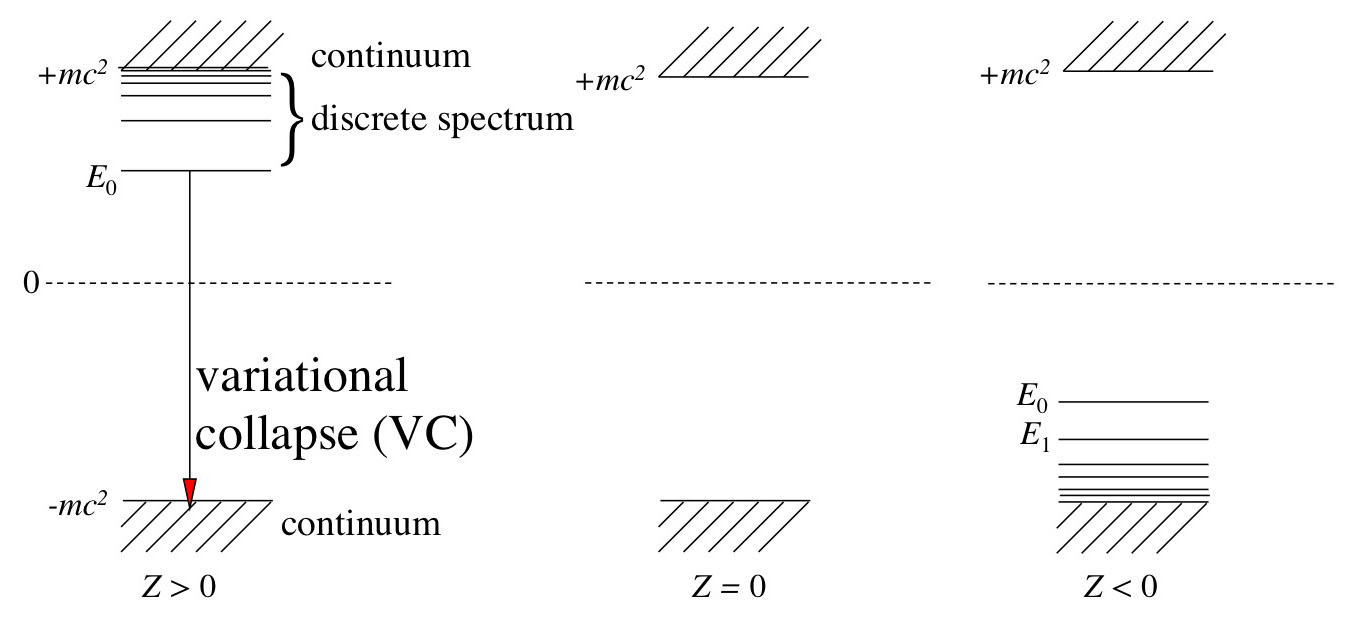
\includegraphics[height=40mm]{figspec.jpg}\\
\caption{Schematic spectrum of the Dirac operator for nuclear charges $Z>0, Z=0$ and $Z<0$.}
\label{fig:spec}
\end{figure*}

For a free spin 1/2 particle the relativistic energy-momentum reveals an energy spectrum of $E\in\{-\infty,-mc^2\}\cup\{+mc^2,\infty\}$. The correct interpretation of the negative energy continuum $\{-\infty,-mc^2\}$ in the spectrum of the Dirac operator has caused many misconceptions to flourish. An electron in a bound or positive energy continuum state could fall into the negative energy continuum (in principle down to $E\rightarrow -\infty$) releasing a photon (variational collapse). We experienced a similar situation in pre-quantum theory where Bohr had to confine electrons in discrete orbits in order not to fall into the positively charged nucleus. Now, here we can do exactly the same (formally) confining electrons to the bound states above the negative energy continuum. The original interpretation of Dirac that the negative energy continuum is completely filled with energy and thus the Pauli principle prevents electrons from entering such states is only of historical importance.\footnote{To cite J. Schwinger 1973: \it The picture of an infinite sea of negative energy electrons is now best regarded as an historical curiosity, and forgotten. Unfortunately, this episode, and discussions of vacuum fluctuations, seem to have left people with the impression that the vacuum, the physical state of nothingness, is actually the scene of wild activity.} Further, if we use the same philosophy for the Klein-Gordon equation for spin-0 particles (bosons), there is no Pauli principle at work preventing {\it all} bosons to go to $E\rightarrow -\infty$. A correct interpretation of these negative energy states comes from Feynman and Stueckelberg in quantum field theory which is discussed in the QED chapter \ref{QED}. If QED effects are ignored and the Dirac equation is treated ``as it is'', we simply have to make sure that a variational collapse is prevented (see section \ref{ME-Dirac}). Formally this can be done by introducing projection operators $\Lambda_{+}$ to the Hilbert sub-space of the states above the negative energy continuum,
\begin{equation}
   D_{+} = \Lambda_{+} D \Lambda_{+}
   \label{DiracBS}
\end{equation}
This will be discussed in more detail in section \ref{ME-Dirac}.

\subsection{\sffamily Solutions for two-particle systems with opposite charge}

\subsubsection{\sffamily The Electron-Nucleus Interaction}
The stationary Dirac equation for an electron in an external (classical) Coulomb field is,
\begin{equation}
   \left\{ c \vec{\alpha} \vec{p} + \beta mc^2 - Zr^{-1} - \left( E + mc^2\right)\right\} \Psi (\vec{r}) = 0
   \label{DiracCoulomb}
\end{equation}
and we shifted the spectrum by $-mc^2$ in order to coincide with the nonrelativistic spectrum from the Schr\"odinger equation. This can formally be done by replacing the $\beta$-matrix, i.e. $\beta'\rightarrow\beta-mc^2$. This leads to two coupled radial differential equations,


In the expression (\ref{DiracCoulomb}) we skipped the center of mass separation, which is rather more difficult for the Dirac equation.\cite{Bechert-Meixner-1935,Breit-1948,Barker-Glover-1955,sapirstein-Yennie-1990} Consider a relativistic effective Hamiltonian treating the nucleus of mass $M$ nonrelativistically\footnote{There is no need for the nucleus to be treated as a fermionic (half-inter nuclear spin) or bosonic (integer nuclear spin) particle (or even down to the quark level), as for example hyperfine effects can be treated effectively in a two-component form.} except for the rest mass energy,
\begin{equation}
   Mc^2 + \frac{P^2}{2M} + \left\{ c \vec{\alpha} \vec{p} + \beta mc^2 - \frac{Z}{|\vec{R}-\vec{r}|} - \left( E + mc^2\right)\right\} \Psi (\vec{R},\vec{r}) = 0
   \label{DiracCoulomb}
\end{equation}



Hydrogen atom with hyperfine structure and QED effects

\subsubsection{\sffamily The Coulomb singularity at the origin and finite extension of the nucleus}
Nuclear charges greater than 137

\subsubsection{\sffamily The Electron-Positron Interaction}
The two-body Dirac equation describing two oppositely charged particles of mass $m_1$ and $m_2$ in a center-of-mass-system interacting via a classical Coulomb interactions is,

Positronium

\subsubsection{\sffamily Other two-particle systems}
Muonium, quarkonium, etc., problem with confinement, MIT bag model

\subsection{\sffamily The classical Breit interaction}
Introduce Breit in a classical way

\subsection{\label{ME-Dirac} \sffamily The multi-electron Dirac equation}
Multi-electron Dirac equation, variational principle, properties

\subsubsection{\sffamily Treating the multi-electron Dirac equation}
Mainly Trond's expertise

\subsection{\label{RelVal}\sffamily Why are relativistic effects large in valence shell of heavy elements?}
Clean up misconceptions

%TWO-COMPONENT FORMS
\section{\label{TwoComp} \sffamily \Large TWO-COMPONENT FORMS}

\subsection{\sffamily Elimination of the small component}
Foly-Wouthuysen, block diagonalizations

\subsection{\sffamily Unitary transformations}
General discussion of unitary transformations

\subsection{\sffamily Matrix formulations}
Mainly Trond's expertise

\subsection{\sffamily Applications}
Examples compare 4- with 2-component

%QUANTUM ELeCTRODYNAMICS
\section{\label{QED} \sffamily \Large QUANTUM ELECTRODYNAMICS}

\subsection{\sffamily Introduction to Feynman diagrams}
Feynman rules


%\begin{fmffile*}{diagram}
%\begin{fmfgraph}(40,25)
%\fmfleft{i1,i2}
%\fmfright{o1,o2}
%\fmf{fermion}q{i1,v1,o1}
%\fmf{fermion}{i2,v2,o2}
%\fmf{photon}{v1,v2}
%\end{fmfgraph}
%\end{fmffile*}


\subsection{\sffamily Vacuum polarization and self-energy}


\subsection{\sffamily Breit interaction from QED}
Frequency dependent Breit, how to treat frequency in CI

\subsection{\sffamily Higher order terms}
Few electron systems only

\subsection{\sffamily Applications}
Examples

%\clearpage

%BEYOND QUANTUM ELeCTRODYNAMICS
\section{\sffamily \Large BEYOND QUANTUM ELECTRODYNAMICS}

\subsection{\sffamily The standard model and beyond}
Introduce the standard model, Problems with standard model (dark matter, dark energy, fundamental constants, ...)

\subsection{\sffamily Electroweak interactions}
Symmetries, CPT theorem, P, CP violation etc., chirality, anapole moment

\subsubsection{\sffamily The electron dipole moment}
Beyond the standard model

%CONCLUSIONS
\subsection{\sffamily \large CONCLUSIONS}
conclusions

%ACKNOWLEDGMENTS
%\subsection*{\sffamily \large ACKNOWLEDGMENTS}
{\footnotesize
{\bf Acknowledgement}: PS is indebted to the Alexander von Humboldt Foundation (Bonn) for financial support 
in terms of a Humboldt Research Award, and to both Gernot Frenking and 
Ralf Tonner (Marburg) for support during his extended stay in Marburg.}
%\clearpage

%%%%%%%%%%%%%%%%%%%%%%%%%%%%%%%%%%%%%%%%%%%%%%%%%%%%%%%%%%%%%%%%%%%%%%%%%%%%%%%%%
% BIBLIOGRAPHY
%%%%%%%%%%%%%%%%%%%%%%%%%%%%%%%%%%%%%%%%%%%%%%%%%%%%%%%%%%%%%%%%%%%%%%%%%%%%%%%%%

% Sort out ref.149,150
\bibliography{dirac}


\end{document}

